\input{hmwrk_header-sol.tex}

%====================================================================
% Commands particular to this file
%====================================================================
\usepackage{graphicx}
\usepackage{multirow}
%\usepackage{bbding} % Allows for Checkmark symbol (\Checkmark with capital is bigger!) and for \XSolidBrush.
%\usepackage[usenames,dvipsnames]{color} % Allows for colors.
%\newcommand{\yes}{{\color{Green}{\Checkmark}}} % Symbol for yes. \Checkmark with capital is bigger!
%\newcommand{\no}{{\color{Red}{\XSolidBrush}}} % Symbol for no. %--------------------------------------------------------------------



\begin{document}

%====================================================================
\homeworktitle{Relations}{Rosen - Chapter 9}

\crossline

\paragraph{Required reading for this list:}
\emph{Discrete Mathematics and Its Applications} (Rosen, 7\textsuperscript{th} Edition):
\begin{itemize}
\item Chapter 9.1: \emph{Relations and Their Properties}
\item Chapter 9.3: \emph{Representing Relations}
\item Chapter 9.4: \emph{Closures of Relations}
\item Chapter 9.5: \emph{Equivalence Relations}
\item Chapter 9.6: \emph{Partial Orderings}
\end{itemize}

\noteondifficultylevel

\crossline

\begin{enumerate}
\item \strmedium (Rosen 9.1-6)
Determine whether the relation $R$ on the set of real numbers is reflexive,
symmetric, antisymmetric, and/or transitive, where $(x,y)\in R$ if and only if:

\begin{multicols}{4}
\begin{enumerate}
\item $x+y=0$
\item $x=\pm y$
\item $x-y$ is rational
\item $x=2y$
\item $xy\geq 0$
\item $xy= 0$
\item $x= 1$
\item $x= 1$ or $y= 1$
\end{enumerate}
\end{multicols}

\solution{
\begin{center}
\begin{tabular}{|l||c|c|c|c|}
\hline
Relation & Reflexive & Symmetric & Antisymmetric & Transitive \\ \hline \hline
(a) $x+y=0$ & \no & \yes & \no & \no \\ \hline
(b) $x=\pm y$ & \yes & \yes & \no & \yes \\ \hline
(c) $x-y$ is rational & \yes & \yes & \no & \yes \\ \hline
(d) $x=2y$ & \no & \no & \yes & \no \\ \hline
(e) $xy\geq 0$ & \yes & \yes & \no & \no \\ \hline
(f) $xy= 0$ & \no & \yes & \no & \no \\ \hline
(g) $x= 1$ & \no & \no & \yes & \yes \\ \hline
(h) $x= 1$ or $y= 1$ & \no & \yes & \no & \no \\ \hline
\end{tabular}
\end{center}
}

\item \strmedium (Rosen 9.1-7)
Determine whether the relation $R$ on the set of all integers
is reflexive, symmetric, antisymmetric, and/or transitive,
where $(x,y)\in R$ if and only if

\begin{multicols}{1}
\begin{enumerate}
\item $x \neq y$.
\item $xy \geq 1$.
\item $x= y+ 1$ or $x = y - 1$.
\item $x= y~(\text{mod }7)$.
\item $x$ is a multiple of $y$.
\item $x$ and $y$ are both negative or both nonnegative.
\item $x= y^{2}$.
\item $x \geq y^{2}$.
\end{enumerate}
\end{multicols}

\solution{
\begin{center}
\begin{tabular}{|l||c|c|c|c|}
\hline
Relation & Reflexive & Symmetric & Antisymmetric & Transitive \\ \hline \hline
(a) $x \neq y$               & \no  & \yes & \no  & \no  \\ \hline
(b) $xy \geq 1$              & \no  & \yes & \no  & \yes \\ \hline
(c) $x= y+ 1$ ou $x = y - 1$ & \no  & \yes & \no  & \no  \\ \hline
(d) $x= y\pmod{7}$    & \yes & \yes & \no  & \yes \\ \hline
(e) $x$ is multiple of $y$    & \yes & \no  & \no  & \yes \\ \hline
(f) $x$ and $y$ are both negative & \multirow{2}{*}{\yes} & \multirow{2}{*}{\yes} & \multirow{2}{*}{\no}  & \multirow{2}{*}{\yes}  \\ 
    or both non-negative   &      &      &      &      \\ \hline
(g) $x= y^{2}$               & \no  & \no  & \yes & \no  \\ \hline
(h) $x \geq y^{2}$           & \no  & \no  & \yes & \yes \\ \hline
\end{tabular}
\end{center}
}

\item \strmedium  (Rosen 9.1-49) Find the error in the ``proof'' of the following ``theorem.''

``Theorem'': Let $R$ be a relation on a set $A$ that is symmetric and transitive. Then $R$ is reflexive.

``Proof'': Let $a\in A$. Take an element $b\in A$ such that $(a, b) \in R$. Because $R$ is symmetric, we also have $(b, a) \in R$. Now using the transitive property, we can conclude that $(a, a) \in R$ because $(a, b) \in R$ and $(b, a) \in R$.

\solution{The second sentence of the proof asks us to ``take an element $b \in A$ such that $(a, b) \in R$.'' There is no guarantee that such an element exists for the taking. This is the only mistake in the proof. If one could be guaranteed that each element in $A$ is related to at least one element, then symmetry and transitivity would indeed imply reflexivity. Without this assumption, however, the proof and the proposition are wrong. As a simple example, take the relation $\varnothing$ on any nonempty set. This relation is vacuously symmetric and transitive, but not reflexive. Here is another counterexample: the relation $\{(1, 1), (1, 2), (2, 1), (2,2)\}$ on the set $\{1,2,3\}$.
}

%\item (Rosen 9.3-15) Let $R$ be the relation represented by the matrix:
%$$
%M_R=\left[ \begin{array}{ccc}
%0&1&0\\
%0&0&1\\
%1&1&0 \end{array} \right]
%$$
%Find the matrices that represent
%\begin{enumerate}
%\item $R^2$
%\item $R^3$
%\item $R^4$
%\end{enumerate}

\item \streasy (Rosen 9.3-19) Draw the directed graphs that represent
the following relations.

\begin{enumerate}
\item ${(1, 2), (1, 3), (1, 4), (2, 3), (2, 4), (3, 4)}$
\item ${(1, 2), (1, 3), (1, 4), (2, 1), (2, 3), (2, 4), (3, 1), (3, 2), (3, 4), (4, 1), (4, 2), (4, 3)}$
\item ${(2, 4), (3, 1), (3, 2), (3, 4)}$
\end{enumerate}

\solution{
\begin{figure}[!htb]
\centering
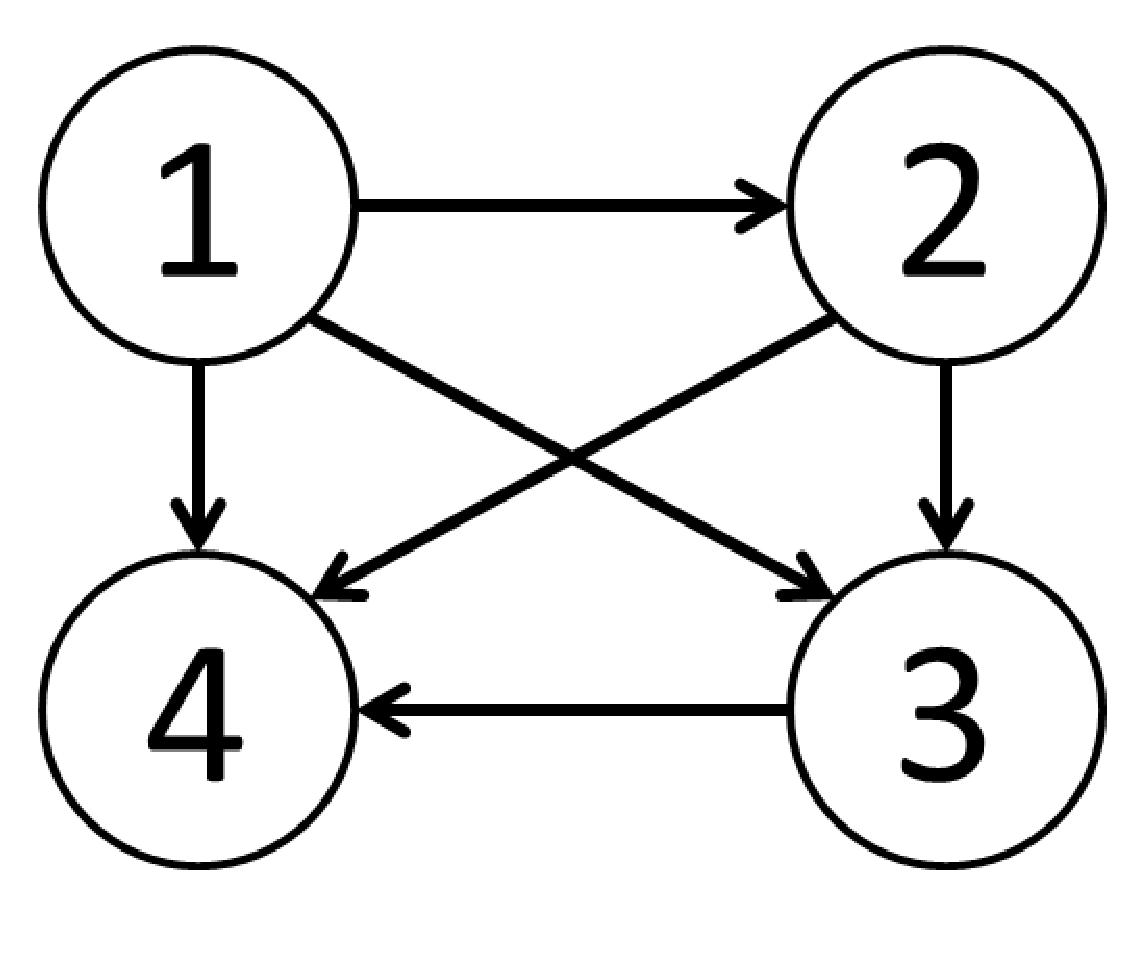
\includegraphics[width=0.2\linewidth]{figs/lista09-9.3-19-a} \hspace{1cm}
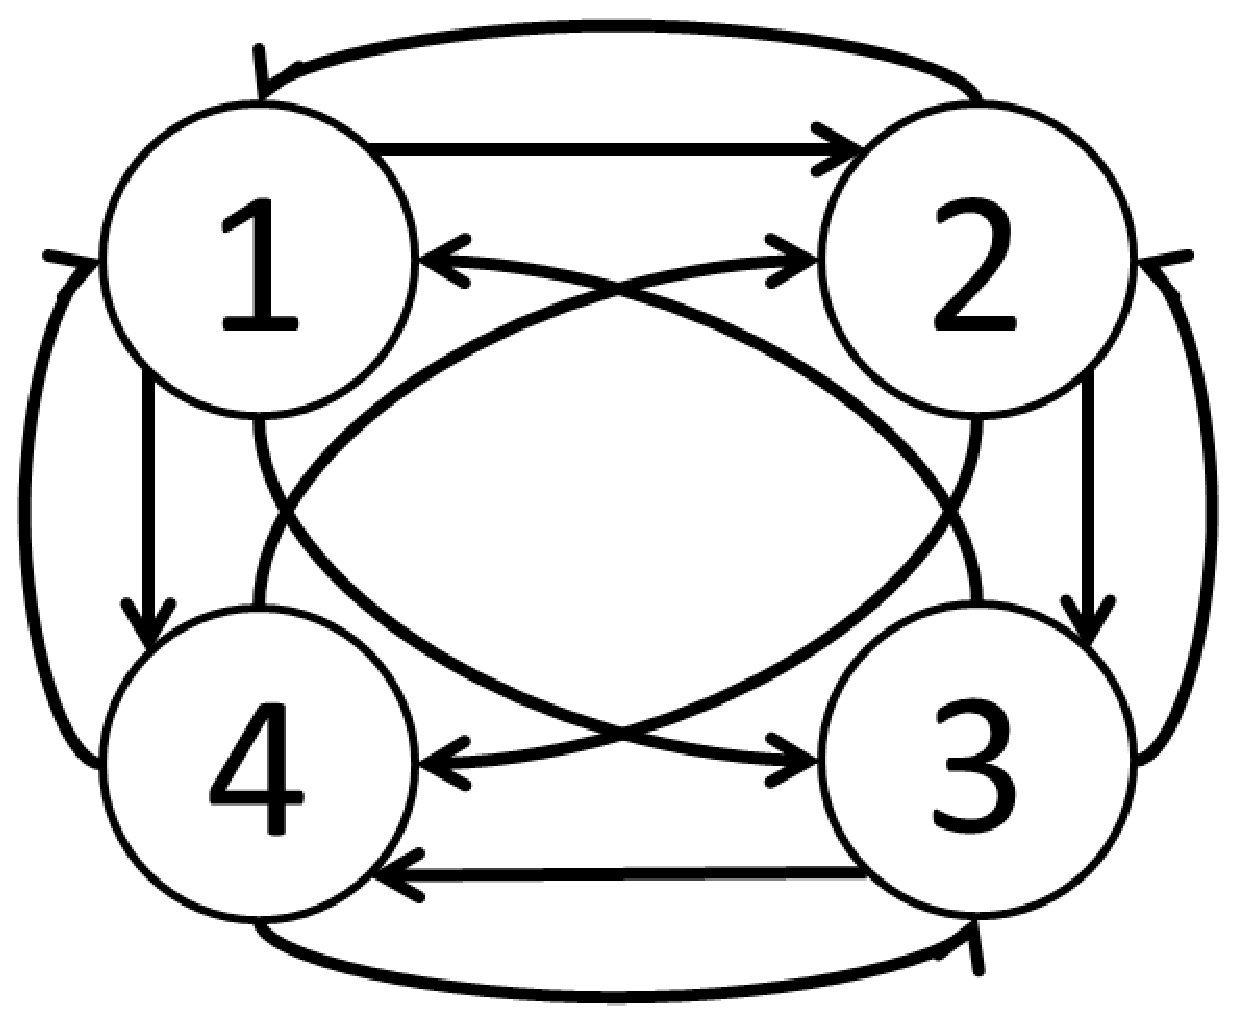
\includegraphics[width=0.2\linewidth]{figs/lista09-9.3-19-b} \hspace{1cm}
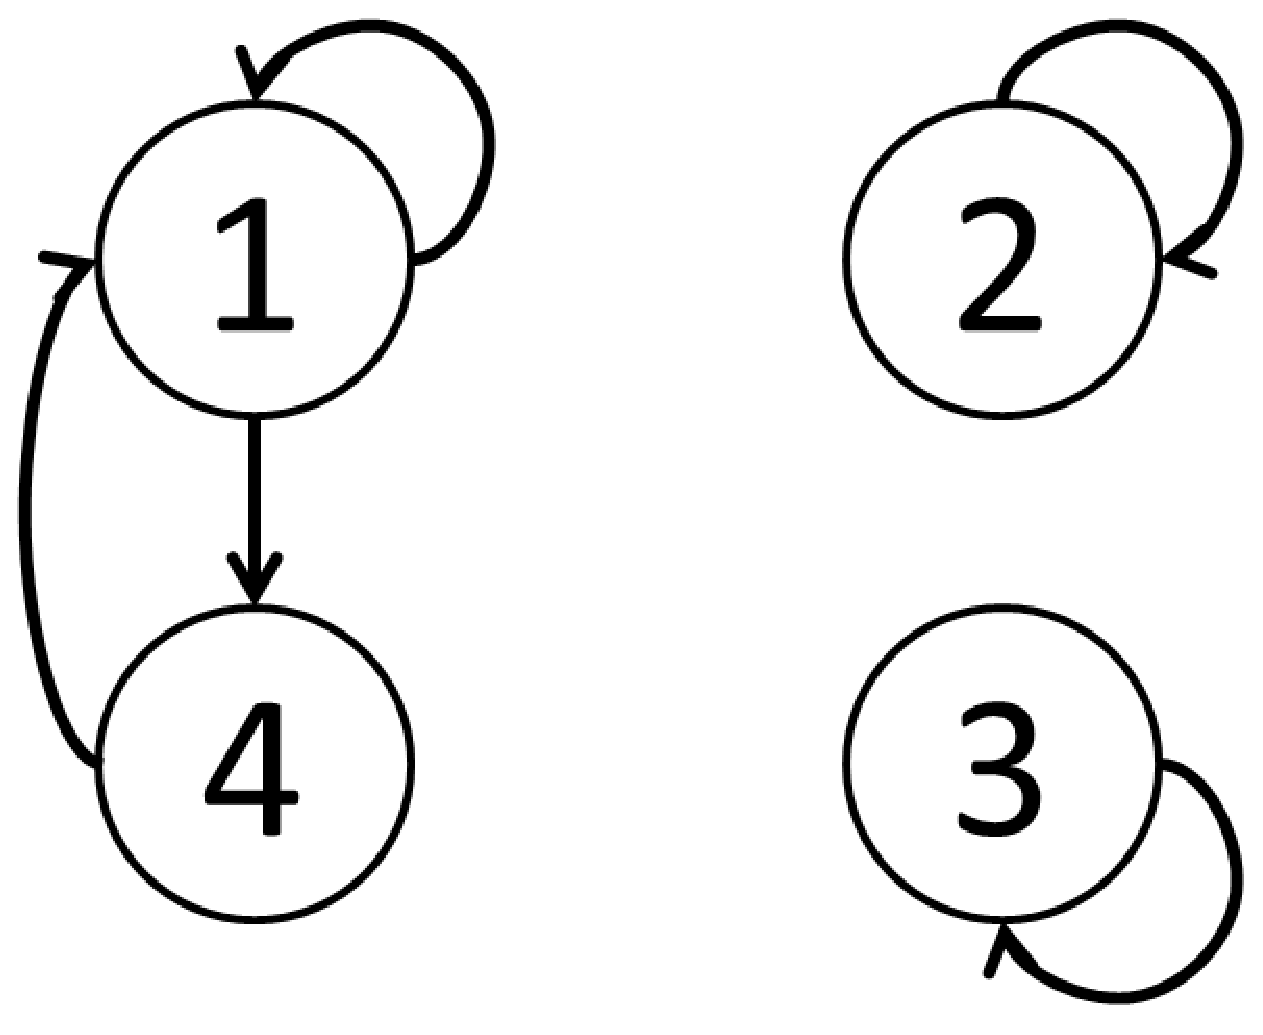
\includegraphics[width=0.2\linewidth]{figs/lista09-9.3-19-c}
\caption{Directed graphs for exercise (Rosen 9.3-19), in order (a), (b), (c).}
\end{figure}
}

\item \streasy (Rosen 9.4-1) Let $R$ be the relation on the set ${0,1,2,3}$ containing
the ordered pairs $(0,1)$, $(1,1)$, $(1,2)$, $(2,0)$, $(2,2)$, and $(3,0)$.
Find the reflexive closure and the symmetric closure of $R$.

\solution{
The reflexive closure of $R$ is ${ (0,0), (0,1), (1,1), (1,2), (2,0), (2,2), (3,0), (3,3) }$
(note that the ordered pairs $(0,0)$ and $(3,3)$ were added to $R$).

The symmetric closure of $R$ is ${ (0,1), (0,2), (0,3), (1,0), (1,1), (1,2), (2,0), (2,1), (2,2), (3,0) }$
(note that the ordered pairs $(1,0)$, $(2,1)$, $(0,2)$, and $(0,3)$ were added to $R$).
}

\item \strmedium (Rosen 9.4-25) Use Algorithm 1 from Section 9.4 to find
the transitive closure of the following relations on ${1,2,3,4}$:
\begin{enumerate}

\item ${ (1,2), (2,1), (2,3), (3,4), (4,1) }$
\solution{
$$
M_{R} = 
\left[
\begin{array}{cccc}
0 & 1 & 0 & 0  \\
1 & 0 & 1 & 0  \\
0 & 0 & 0 & 1  \\
1 & 0 & 0 & 0 
\end{array}
\right]
\quad
M_{R}^{[2]} = 
\left[
\begin{array}{cccc}
1 & 0 & 1 & 0 \\  
0 & 1 & 0 & 1 \\ 
1 & 0 & 0 & 0 \\ 
0 & 1 & 0 & 0 
\end{array}
\right]
\quad
M_{R}^{[3]} = 
\left[
\begin{array}{cccc}
0 & 1 & 0 & 1 \\  
1 & 0 & 1 & 0 \\  
0 & 1 & 0 & 0 \\  
1 & 0 & 1 & 0   
\end{array}     
\right] \\
$$
$$
M_{R}^{[4]} = 
\left[
\begin{array}{cccc}
1 & 0 & 1 & 0 \\  
0 & 1 & 0 & 1 \\  
1 & 0 & 1 & 0 \\  
0 & 1 & 0 & 1    
\end{array}
\right]
\quad
M_{R}^{*} = 
\left[
\begin{array}{cccc}
1 & 1 & 1 & 1  \\
1 & 1 & 1 & 1  \\
1 & 1 & 1 & 1  \\  
1 & 1 & 1 & 1   
\end{array}
\right]
$$
Hence the transitive closure of $R$ is
$R^{*} = \{ (1,1), \allowbreak (1,2), \allowbreak (1,3), \allowbreak (1,4), 
\allowbreak (2,1), \allowbreak (2,2), \allowbreak (2,3), \allowbreak (2,4), 
\allowbreak (3,1), \allowbreak (3,2), \allowbreak (3,3), \allowbreak (3,4), 
\allowbreak (4,1), \allowbreak (4,2), \allowbreak (4,3), \allowbreak (4,4) 
\}$.
}

\item $\{ (2,1), (2,3), (3,1), (3,4), (4,1), (4,3) \}$
\solution{
$$
M_{R} = 
\left[
\begin{array}{cccc}
0 & 0 & 0 & 0  \\
1 & 0 & 1 & 0  \\
1 & 0 & 0 & 1  \\
1 & 0 & 1 & 0 
\end{array}
\right]
\quad
M_{R}^{[2]} = 
\left[
\begin{array}{cccc}
0 & 0 & 0 & 0  \\
1 & 0 & 0 & 1  \\
1 & 0 & 1 & 0  \\
1 & 0 & 0 & 1 
\end{array}
\right]
\quad
M_{R}^{[3]} = 
\left[
\begin{array}{cccc}
0 & 0 & 0 & 0  \\
1 & 0 & 1 & 0  \\
1 & 0 & 0 & 1  \\
1 & 0 & 1 & 0   
\end{array}     
\right] \\
$$
$$
M_{R}^{[4]} = 
\left[
\begin{array}{cccc}
1 & 0 & 1 & 0 \\  
0 & 1 & 0 & 1 \\  
1 & 0 & 1 & 0 \\  
0 & 1 & 0 & 1  
\end{array}
\right]
\quad
M_{R}^{*} = 
\left[
\begin{array}{cccc}
0 & 0 & 0 & 0  \\
1 & 0 & 1 & 1  \\
1 & 0 & 1 & 1  \\  
1 & 0 & 1 & 1   
\end{array}
\right]
$$
Hence the transitive closure of $R$ is
$R^{*} = \{ (2,1), \allowbreak (2,3), \allowbreak (2,4), 
(3,1), \allowbreak (3,3), \allowbreak (3,4), 
(4,1), \allowbreak (4,3), \allowbreak (4,4)
\}$.
}

\end{enumerate}

\item \strmedium (Rosen 9.4-26) Use Algorithm 1 from Section 9.4 to find
the transitive closure of the following relations on ${a,b,c,d,e}$:
\begin{enumerate}
\item $\{(a,c), (b,d), (c,a), (d,b), (e,d)\}$
\solution{
$$
M_{R} = 
\left[
\begin{array}{ccccc}
0 & 0 & 1 & 0 & 0 \\
0 & 0 & 0 & 1 & 0 \\
1 & 0 & 0 & 0 & 0 \\
0 & 1 & 0 & 0 & 0 \\
0 & 0 & 0 & 1 & 0
\end{array}
\right]
\quad
M_{R}^{[2]} = 
\left[
\begin{array}{ccccc}
1 & 0 & 0 & 0 & 0 \\
0 & 1 & 0 & 0 & 0 \\
0 & 0 & 1 & 0 & 0 \\
0 & 0 & 0 & 1 & 0 \\
0 & 1 & 0 & 0 & 0 
\end{array}
\right]
\quad
M_{R}^{[3]} = 
\left[
\begin{array}{ccccc}
0 & 0 & 1 & 0 & 0 \\
0 & 0 & 0 & 1 & 0 \\
1 & 0 & 0 & 0 & 0 \\
0 & 1 & 0 & 0 & 0 \\
0 & 0 & 0 & 1 & 0 
\end{array}
\right] \\
$$

$$
M_{R}^{[4]} = 
\left[
\begin{array}{ccccc}
1 & 0 & 0 & 0 & 0 \\
0 & 1 & 0 & 0 & 0 \\
0 & 0 & 1 & 0 & 0 \\
0 & 0 & 0 & 1 & 0 \\
0 & 1 & 0 & 0 & 0 
\end{array}
\right]
\quad
M_{R}^{[5]} = 
\left[
\begin{array}{ccccc}
0 & 0 & 1 & 0 & 0 \\
0 & 0 & 0 & 1 & 0 \\
1 & 0 & 0 & 0 & 0 \\
0 & 1 & 0 & 0 & 0 \\
0 & 0 & 0 & 1 & 0 
\end{array}
\right]
\quad
M_{R}^{*} = 
\left[
\begin{array}{ccccc}
1 & 0 & 1 & 0 & 0 \\
0 & 1 & 0 & 1 & 0 \\
1 & 0 & 1 & 0 & 0 \\
0 & 1 & 0 & 1 & 0 \\  
0 & 1 & 0 & 1 & 0  
\end{array}
\right]
$$
Hence the transitive closure of $R$ is:
$R^{*} = \{ (a,a), \allowbreak (a,c), \allowbreak (b,b), \allowbreak (b,d), \allowbreak (c,a),
\allowbreak (c,c), \allowbreak (d,b), \allowbreak (d,d), \allowbreak (e,b), \allowbreak (e,d)
\}$.
}


\item $\{(a,e), (b,a), (b,d), (c,d), (d,a), (d,c), (e,a), (e,b) (e,c), (e,e)\}$
\solution{
$$
M_{R} = 
\left[
\begin{array}{ccccc}
0 & 0 & 0 & 0 & 1 \\  
1 & 0 & 0 & 1 & 0 \\  
0 & 0 & 0 & 1 & 0 \\  
1 & 0 & 1 & 0 & 0 \\  
1 & 1 & 1 & 0 & 1
\end{array}
\right]
\quad
M_{R}^{[2]} = 
\left[
\begin{array}{ccccc}
1 & 1 & 1 & 0 & 1 \\
1 & 0 & 1 & 0 & 1 \\
1 & 0 & 1 & 0 & 0 \\
0 & 0 & 0 & 1 & 1 \\
1 & 1 & 1 & 1 & 1 
\end{array}
\right]
\quad
M_{R}^{[3]} = 
\left[
\begin{array}{ccccc}
1 & 1 & 1 & 1 & 1 \\
1 & 1 & 1 & 1 & 1 \\
0 & 0 & 0 & 1 & 1 \\
1 & 1 & 1 & 0 & 1 \\
1 & 1 & 1 & 1 & 1 
\end{array}
\right] \\
$$

$$
M_{R}^{[4]} = 
\left[
\begin{array}{ccccc}
1 & 1 & 1 & 1 & 1 \\
1 & 1 & 1 & 1 & 1 \\
1 & 1 & 1 & 0 & 1 \\
1 & 1 & 1 & 1 & 1 \\
1 & 1 & 1 & 1 & 1 
\end{array}
\right]
\quad
M_{R}^{[5]} = 
\left[
\begin{array}{ccccc}
1 & 1 & 1 & 1 & 1 \\
1 & 1 & 1 & 1 & 1 \\
1 & 1 & 1 & 1 & 1 \\
1 & 1 & 1 & 1 & 1 \\
1 & 1 & 1 & 1 & 1 
\end{array}
\right]
\quad
M_{R}^{*} = 
\left[
\begin{array}{ccccc}
1 & 1 & 1 & 1 & 1 \\
1 & 1 & 1 & 1 & 1 \\
1 & 1 & 1 & 1 & 1 \\
1 & 1 & 1 & 1 & 1 \\
1 & 1 & 1 & 1 & 1 
\end{array}
\right]
$$
Hence the transitive closure of $R$ is: 
$R^{*} = \{ (a,a), \allowbreak (a,b), \allowbreak (a,c), \allowbreak (a,d), \allowbreak (a,e),
\allowbreak (b,a), \allowbreak (b,b), \allowbreak (b,c), \allowbreak (b,d), \allowbreak (b,e),
\allowbreak (c,a), \allowbreak (c,b), \allowbreak (c,c), \allowbreak (c,d), \allowbreak (c,e),
\allowbreak (d,a), \allowbreak (d,b), \allowbreak (d,c), \allowbreak (d,d), \allowbreak (d,e),
\allowbreak (e,a), \allowbreak (e,b), \allowbreak (e,c), \allowbreak (e,d), \allowbreak (e,e) 
\}$.
}

\solution{
}
\end{enumerate}

\item  (Rosen 9.4-35)
Show that the closure with respect to the property $P$ of the relation $R = \{(0, 0), (0, 1), (1, 1), (2, 2)\}$ on the set $\{0, 1, 2\}$ does not exist if $P$ is the property:
\begin{itemize}
\item[a)]  \streasy ``is not reflexive.''
\item[b)] \strhard ``has an odd number of elements.''
\end{itemize}
\solution{
\begin{itemize}
\item[a)] No relation that contains $R$ is not reflexive, since $R$ already contains all the pairs $(0, 0), (1, 1), (2, 2)$. Therefore there is no ``non reflexive'' closure of $R$.
\item[b)] Suppose $S$ were the closure of $R$ with respect to this property. Since $R$ does not have an odd number of elements, $S \not= R$, so $S$ must be a proper superset of $R$. Clearly $S$ cannot have more than 5 elements, for if it did, then any subset of $S$ consisting of $R$ and one element of $S - R$ would be a proper subset of $S$ with the property; this would violate the requirement that $S$ be a subset of every superset of $R$ with the property. Thus $S$ must have exactly 5 elements. Let $T$ be another superset of $R$ with 5 elements (there are $9 - 4 = 5$ such sets in all). Thus $T$ has the property, but $S$ is not a subset of $T$. This contradicts the definition. Therefore our original assumption was faulty, and the closure does not exist.
\end{itemize}
}

\item \strmedium (Rosen 9.5-1)
Which of these relations on the set $\{0,1,2,3\}$ are equivalence relations?
For the relations that are not equivalence relations, indicate which properties 
of an equivalence relation they do not satisfy.

\begin{enumerate}
\item $\{(0,0),(1,1),(2,2),(3,3)\}$
\solution{
This is an equivalence relation.
}

\item $\{(0,2),(2,0),(2,2),(2,3),(3,2),(3,3)\}$
\solution{
It is not reflexive and not transitive.
}

\item $\{(0,0),(1,1),(1,2),(2,1),(2,2),(3,3)\}$
\solution{
This is an equivalence relation.
}

\item $\{(0,0),(1,1),(1,3),(2,2),(2,3),(3,1),(3,2),(3,3)\}$
\solution{
It is not transitive.
}

\item $\{(0,0),(0,1),(0,2),(1,0),(1,1),(1,2),(2,0),(2,2),(3,3)\}$
\solution{
It is not symmetric and not transitive.
}
\end{enumerate}

\item \strmedium (Rosen 9.5-3)
Which of these relations on the set of all functions from $\mathbb{Z}$ 
to $\mathbb{Z}$ are equivalence relations?
For those that are not equivalence relations, indicate which properties 
they fail to satisfy.

\begin{enumerate}
\item $\{ (f,g) \mid f(1) = g(1) \}$
\solution{
This is an equivalence relation.
}

\item $\{ (f,g) \mid  f(0) = g(0) \text{ or } f(1) = g(1) \}$
\solution{
It is not transitive.
}

\item $\{ (f,g) \mid f(x) - g(x) = 1 \text{ for all } x \in \mathbb{Z} \}$
\solution{
It is not reflexive, not symmetric, and not transitive.
}

\item $\{ (f,g) \mid \text{ there exists $c \in \mathbb{Z}$ such that for all $x \in \mathbb{Z}$, } f(x) - g(x) = c \}$
\solution{
This is an equivalence relation.
}

\item $\{ (f,g) \mid f(0) = g(1) \text{ and } f(1) = g(0) \}$
\solution{
It is not reflexive and not transitive.
}
\end{enumerate}

\item \strhard (Rosen 9.5-15) Let $R$ be the relation on ordered pairs of positive 
integers defined by $((a,b),(c,d)) \in R$ if and only if $a+d = b+c$. 
Show that $R$ is an equivalence relation.

\solution{
We need to verify that $R$ is reflexive, symmetric, and transitive.

\textbf{Reflexivity:} For any positive integers $a,b$, we have $a+b = a+b$, 
so $((a,b),(a,b)) \in R$. Hence, $R$ is reflexive.

\textbf{Symmetry:} If $((a,b),(c,d)) \in R$, then $a+d = b+c$. 
This implies $c+b = d+a$, so $((c,d),(a,b)) \in R$. Thus, $R$ is symmetric.

\textbf{Transitivity:} Suppose $((a,b),(c,d)) \in R$ and $((c,d),(e,f)) \in R$, 
so $a+d = b+c$ and $c+f = d+e$. Adding and rearranging gives $a+f = b+e$, 
so $((a,b),(e,f)) \in R$. Therefore, $R$ is transitive.
}

\item \strmedium (Rosen 9.6-3) Let $S$ be the set of all people in the world.
Determine whether $(S,R)$ is a poset when $R$ is the relation on $S$ defined by:
\begin{enumerate}
\item $a$ is taller than $b$?
\solution{
No, because the relation is not reflexive (no one is taller than themselves) 
and not antisymmetric (two people could have the same height).
}

\item $a$ is not taller than $b$?
\solution{
No, because the relation is not antisymmetric (two people of the same height 
violate antisymmetry).
}

\item $a=b$ or $a$ is an ancestor of $b$?
\solution{
Yes, because this relation is reflexive, antisymmetric, and transitive.
}

\item $a$ and $b$ have a friend in common?
\solution{
No, because the relation is not reflexive, not antisymmetric, and not transitive.
}
\end{enumerate}

\item \strmedium (Rosen 9.6-4) Let $S$ be the set of all people and $(a,b)\in R$. 
$(S,R)$ is a poset if:
\begin{enumerate}
\item $a$ is not shorter than $b$?
\solution{
No, it is not antisymmetric: two people of equal height violate antisymmetry.
}

\item $a$ weighs more than $b$?
\solution{
No, it is not reflexive (no one weighs more than themselves).
}

\item $a=b$ or $a$ is a descendant of $b$?
\solution{
Yes, the relation is reflexive, antisymmetric, and transitive.
}

\item $a$ and $b$ do not have a friend in common?
\solution{
No, it is not reflexive, not antisymmetric, and not transitive.
}
\end{enumerate}

\item \strmedium (Rosen 9.6-5) Which of the following sets are posets?
\begin{multicols}{3}
\begin{enumerate}
\item $(\mathbb{Z},=)$
\item $(\mathbb{Z},\neq)$
\item $(\mathbb{Z},\geq)$
\item $(\mathbb{Z},\not{\mid})$
\end{enumerate}
\end{multicols}

\solution{
\begin{enumerate}
\item $(\mathbb{Z},=)$ is a poset because equality is reflexive, antisymmetric, and transitive.
\item $(\mathbb{Z},\neq)$ is not a poset because it is not reflexive, antisymmetric, or transitive.
\item $(\mathbb{Z},\geq)$ is a poset because $\geq$ is reflexive, antisymmetric, and transitive.
\item $(\mathbb{Z},\not{\mid})$ is not a poset because it is not reflexive, antisymmetric, or transitive.
\end{enumerate}
}

\item \strmedium (Rosen 9.6-6) Which of the following sets are posets?
\begin{multicols}{4}
\begin{enumerate}
\item $(\mathbb{R},=)$
\item $(\mathbb{R},<)$
\item $(\mathbb{R},\leq)$
\item $(\mathbb{R},\neq)$
\end{enumerate}
\end{multicols}

\solution{
\begin{enumerate}
\item $(\mathbb{R},=)$ is a poset because equality is reflexive, antisymmetric, and transitive.
\item $(\mathbb{R},<)$ is not a poset because $<$ is not reflexive.
\item $(\mathbb{R},\leq)$ is a poset because $\leq$ is reflexive, antisymmetric, and transitive.
\item $(\mathbb{R},\neq)$ is not a poset because it is not reflexive, antisymmetric, or transitive.
\end{enumerate}
}

\item \streasy (Rosen 9.6-17) Determine the lexicographic order of the following $n$-tuples:

\begin{multicols}{3}
\begin{enumerate}
\item $(1,1,2),(1,2,1)$

\item $(0,1,2,3),(0,1,3,2)$

\item $(1,0,1,0,1),(0,1,1,1,0)$
\end{enumerate}
\end{multicols}

\solution{
\begin{multicols}{3}
\begin{enumerate}
\item $(1,1,2) \prec (1,2,1)$.

\item $(0,1,2,3) \prec (0,1,3,2)$.

\item $(1,0,1,0,1) \succ (0,1,1,1,0)$.
\end{enumerate}
\end{multicols}
}

\item \strmedium (Rosen 9.6-22) Draw the Hasse diagram for the divisibility relation over:

\begin{multicols}{2}
\begin{enumerate}
\item $\{1,2,3,4,5,6\}$
\item $\{1,3,9,27,81,243\}$
\end{enumerate}
\end{multicols}

\solution{
\begin{figure}[!htb]
\centering
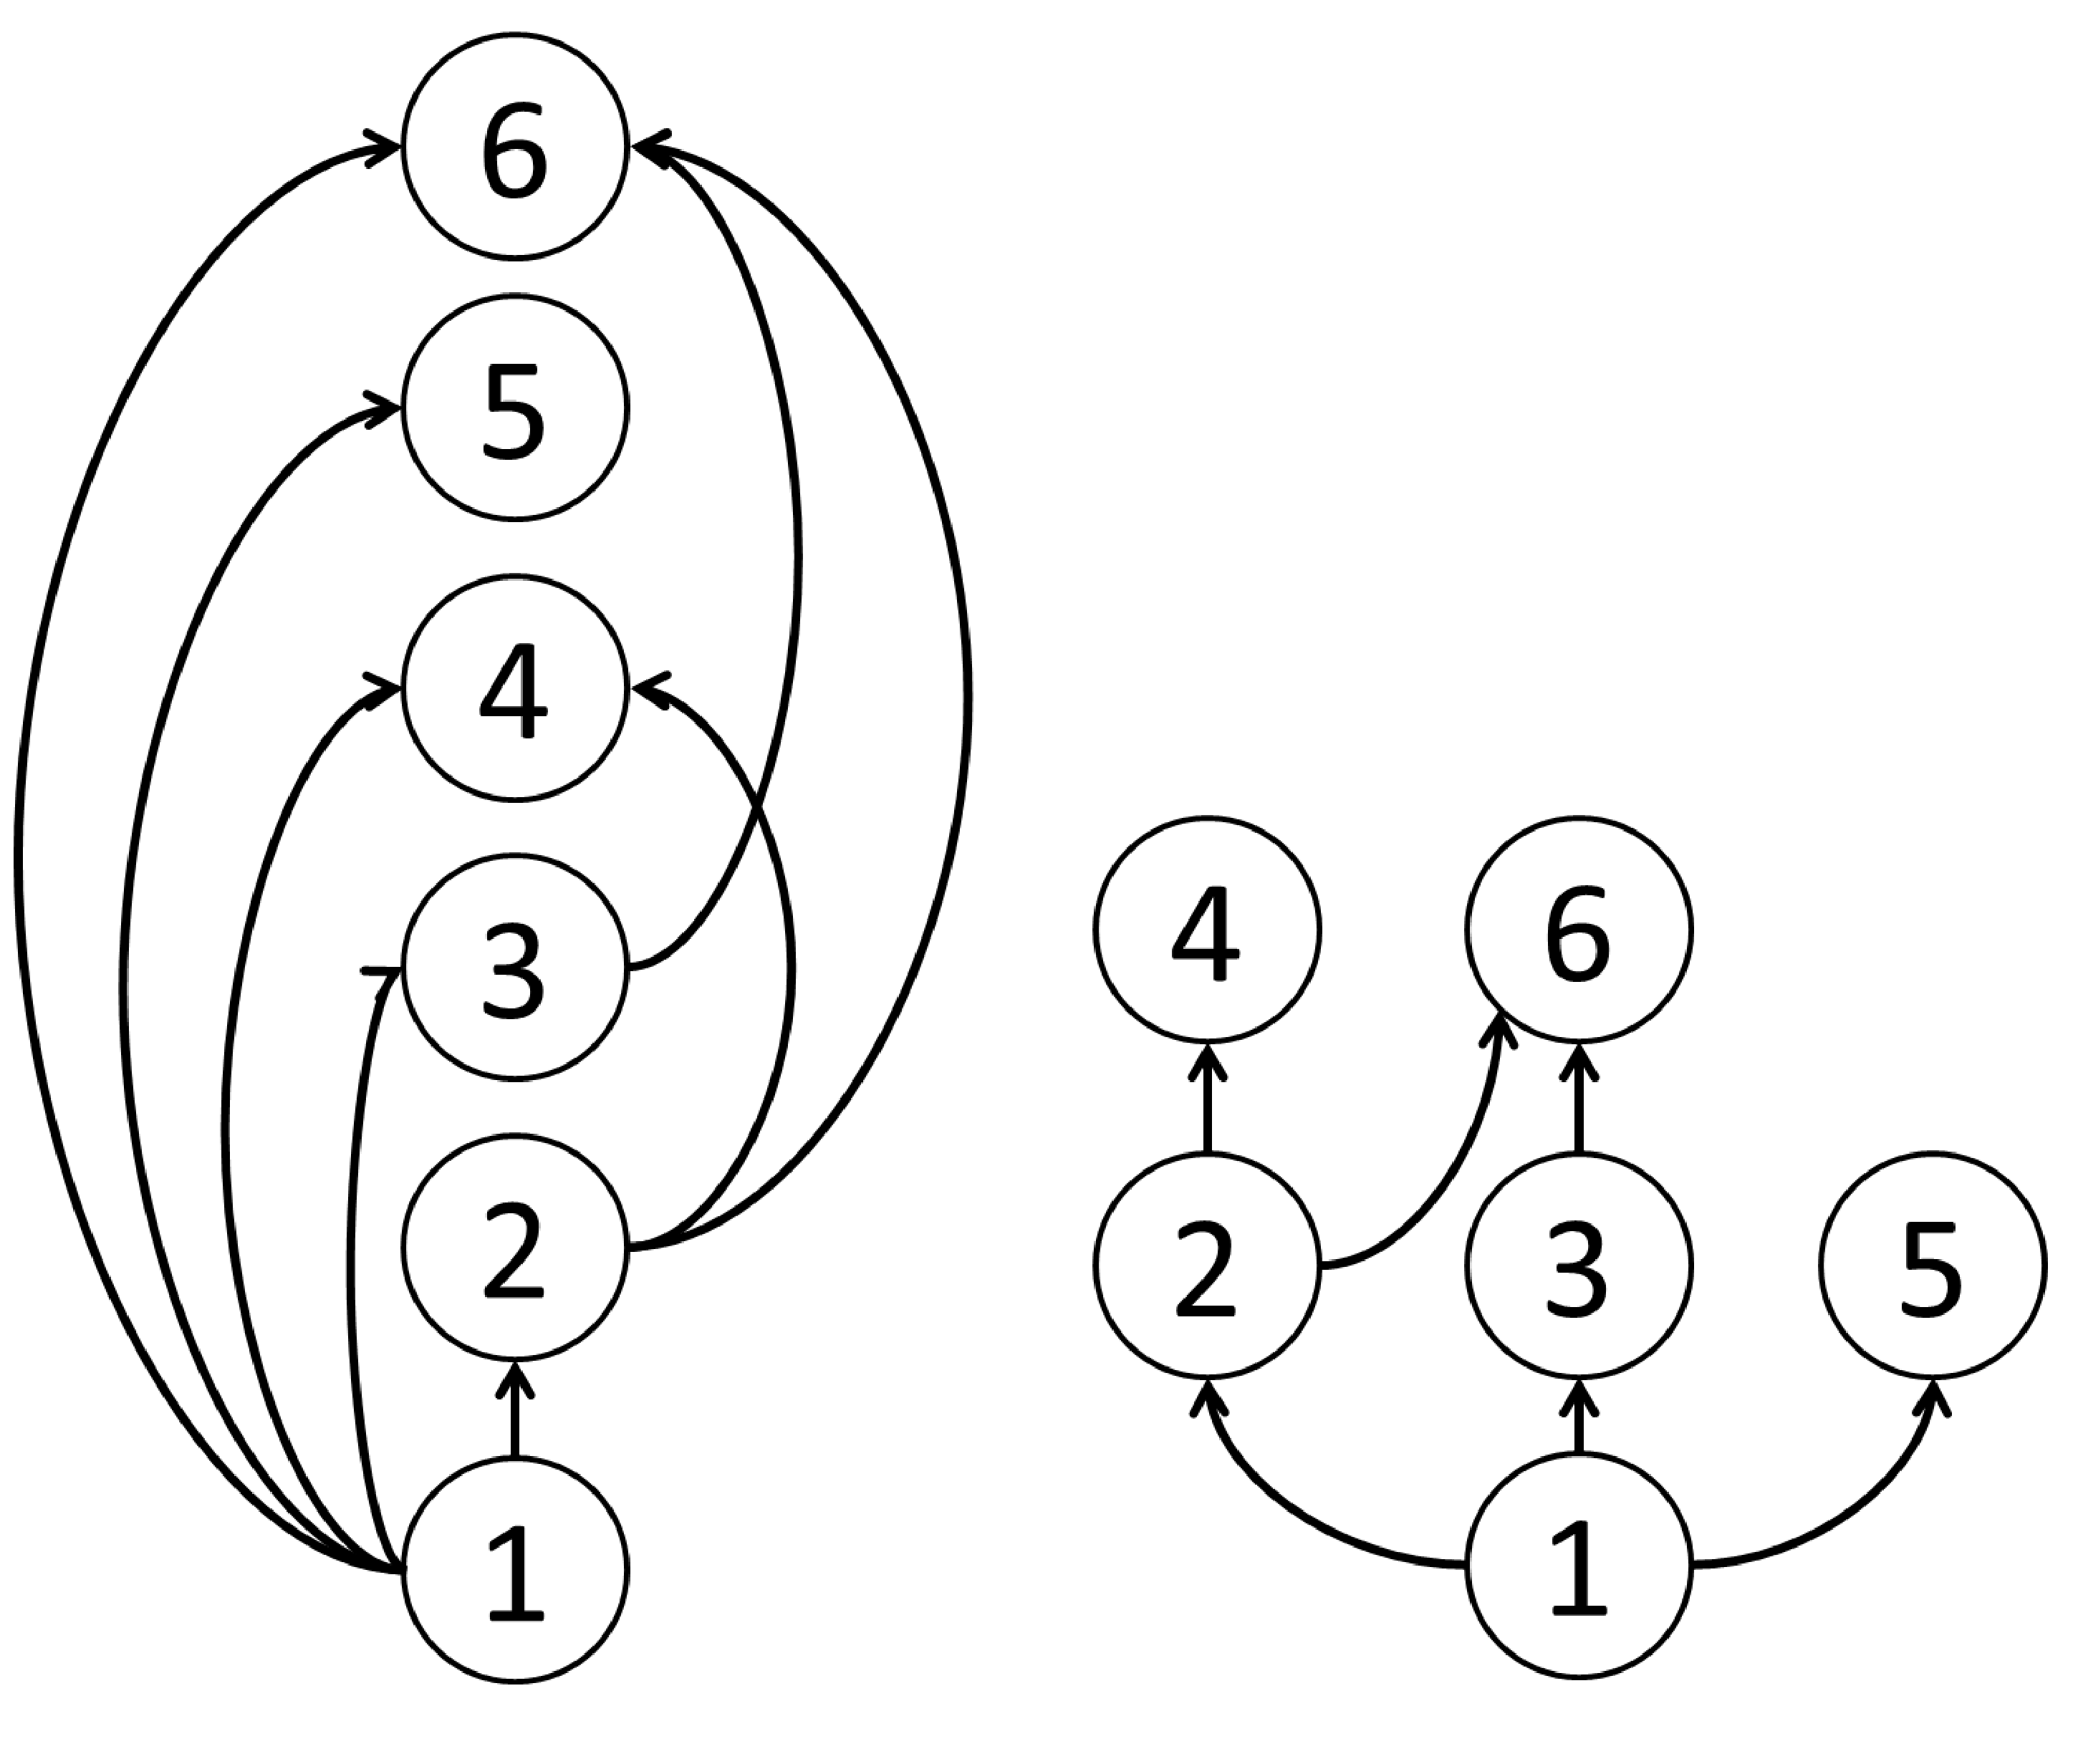
\includegraphics[width=0.3\linewidth]{figs/lista09-9.6-22-a} \hspace{1cm}
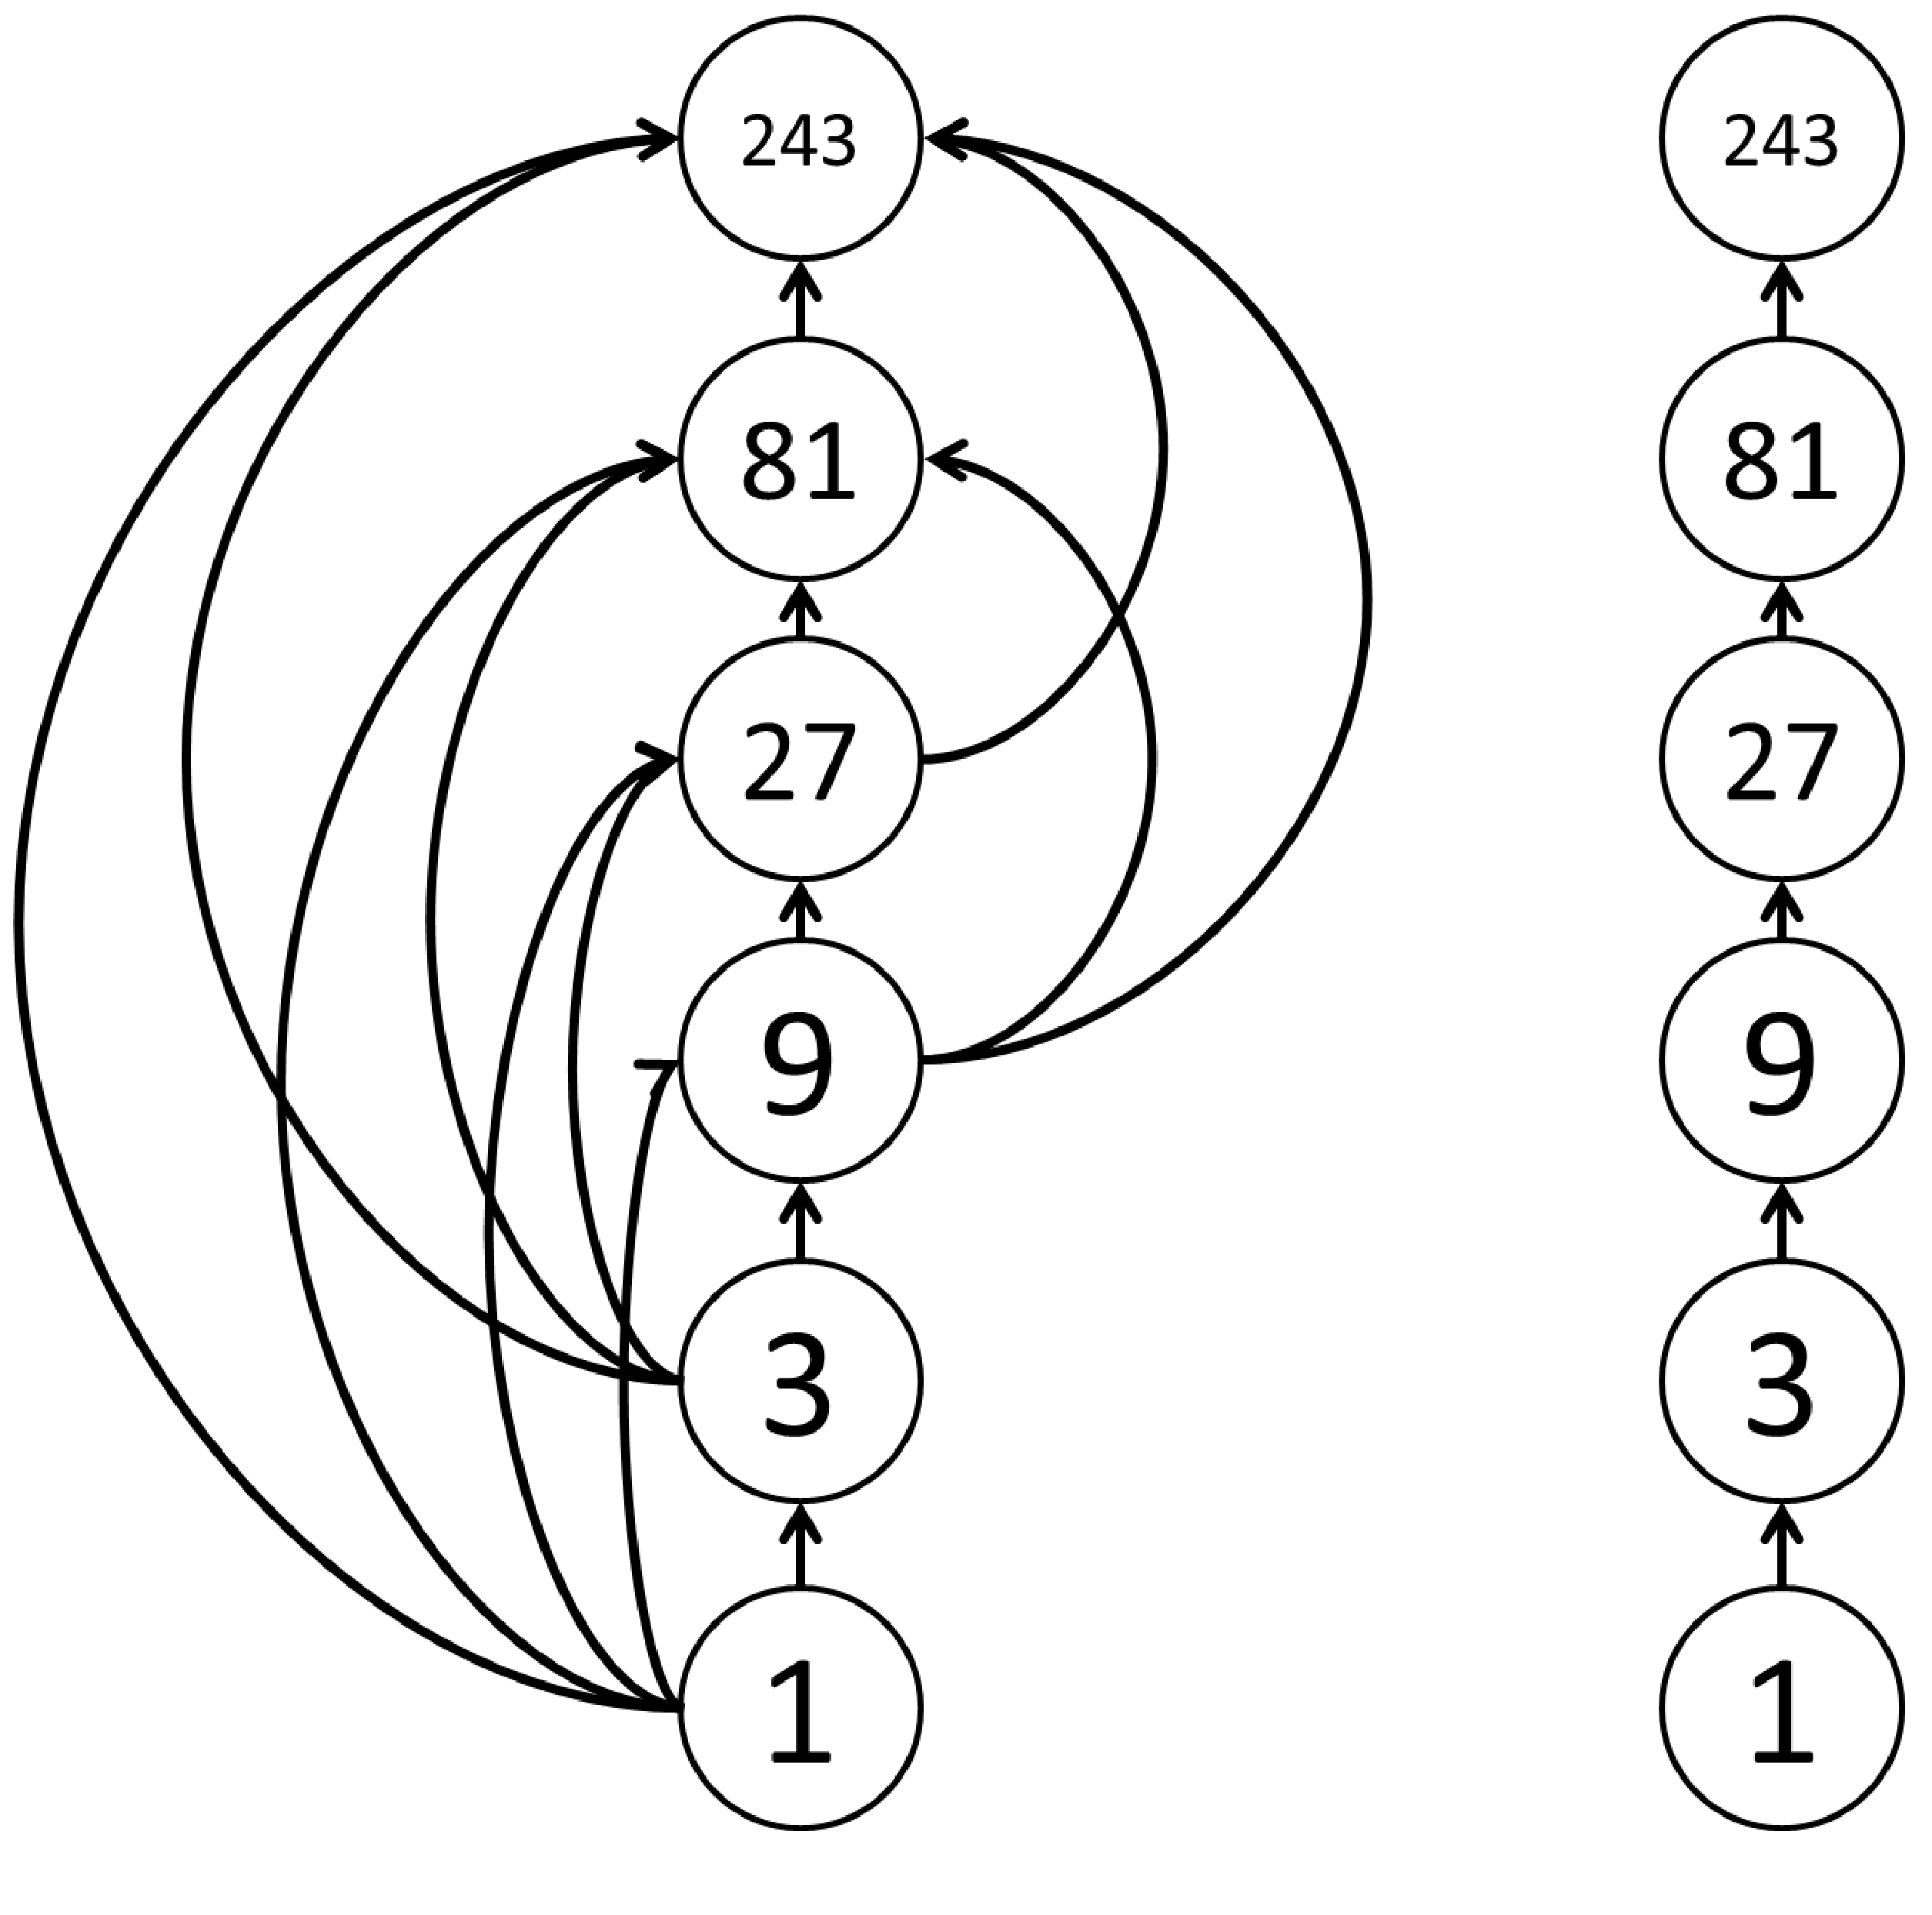
\includegraphics[width=0.3\linewidth]{figs/lista09-9.6-22-b} 
\caption{Original directed graphs and Hasse diagrams for exercise (Rosen 9.6-22), in order (a), (b).}
\end{figure}
}

\item \strmedium Let $A = \{2, 4\}$ and $B = \{6, 8, 10\}$, and define binary relations $R$ and $S$ as:
\begin{align*}
\forall (x,y) \in A \times B, xRy  &\Leftrightarrow  x \mid y \\
\forall (x,y) \in A \times B, xSy  &\Leftrightarrow  y-4=x
\end{align*}
List the ordered pairs in $A \times B$, $R$, $S$, $R \cup S$, and $R \cap S$.

\solution{
\begin{center}
\begin{tabular}{|c||c c c c c c|}
\hline
$A \times B$	& $(2,6)$ & $(2,8)$ & $(2,10)$ & $(4,6)$ & $(4,8)$ & $(4,10)$ \\ \hline \hline
$R$ 			& $(2,6)$ & $(2,8)$ & $(2,10)$ & \no     & $(4,8)$ & \no      \\ \hline
$S$				& $(2,6)$ & \no   	& \no      & \no     & $(4,8)$ & \no      \\ \hline
$R \cup S$		& $(2,6)$ & $(2,8)$ & $(2,10)$ & \no     & $(4,8)$ & \no      \\ \hline
$R \cap S$		& $(2,6)$ & \no   	& \no      & \no     & $(4,8)$ & \no     \\ \hline
\end{tabular}
\end{center}
}

\item \strhard Let $D$ be a relation on $\mathbb{R}^2$ defined as:
\begin{equation*}
\forall (x,y) \in \mathbb{R}^{2}, xDy  \Leftrightarrow  xy \geq 0.
\end{equation*}
Determine whether $D$ is reflexive, symmetric, and transitive.

\solution{
\begin{itemize}
\item \textbf{Reflexive:} $xx = x^2 \geq 0$ for all real $x$, so $D$ is reflexive.

\item \textbf{Symmetric:} If $xy \geq 0$, then $yx \geq 0$, so $D$ is symmetric.

\item \textbf{Transitive:} Take $x=-1$, $y=0$, $z=1$. We have $xy = 0 \geq 0$ and $yz = 0 \geq 0$, but $xz = -1 < 0$. Hence $D$ is not transitive.
\end{itemize}
}

\item \label{item:Loureiro-1} \strmedium
\textbf{Composition of relations:} If $R$ is a relation from $A$ to $B$ and $S$ is a relation from $B$ to $C$, the composition $S \circ R$ consists of pairs $(a,c)$ such that there exists $b \in B$ with $(a,b)\in R$ and $(b,c)\in S$.

Find $S \circ R$ where $R: \{1,2,3\} \to \{1,2,3,4\}$ with 
$R = \{ (1,1),(1,4),(2,3),(3,1),(3,4) \}$ and $S: \{1,2,3,4\} \to \{0,1,2\}$ with 
$S = \{ (1,0),(2,0),(3,1),(3,2),(4,1) \}$.

\solution{
$S \circ R = \{ (1,0), (1,1), (2,1), (2,2), (3,0), (3,1) \}$.
\begin{figure}[!htb]
\centering
\includegraphics[width=0.25\textwidth]{figs/lista09_Loureiro_1}
\caption{Figure for the relations in exercise~\ref{item:Loureiro-1}}
\label{fig:Loureiro-1}
\end{figure}
}

\end{enumerate}

\end{document}

